%======================================================================
\subsection{BW-ECD-05 --- Built, 30 Oct: KiCad parts in the Standard Libraries vault}\label{sec:ecd05-built}
%======================================================================

You asked to tie the KiCad work into the vault: an electrical part lives in the Standard Libraries like any other
standard part, its electrical design opens in KiCad, and its 3D model opens in Keystone. Built in five commits
(\code{9b97342d}, \code{dcac4bb0}, \code{345f47d8}, \code{bcfeb115}, \code{1afbf810}): the engine is FreeCAD-free in
\file{addons/BruceWorx/bruceworx/ecad\_vault.py} (with small additions to \file{pdm\_workspace.py},
\file{kicad\_bridge.py} and \file{cli.py}); the Keystone side is in \file{src/Mod/BruceWorx/bruceworx\_board.py} and
\file{bruceworx\_board\_gui.py}, with a four-line hook in the vault client. Your 23 Oct decisions stand (our own
\code{kicad-cli} bridge, one PCBA BOM line, materials by footprint library, KiCad's render as the thumbnail, only you
edit boards).

\begin{figure}[!htbp]
\centering
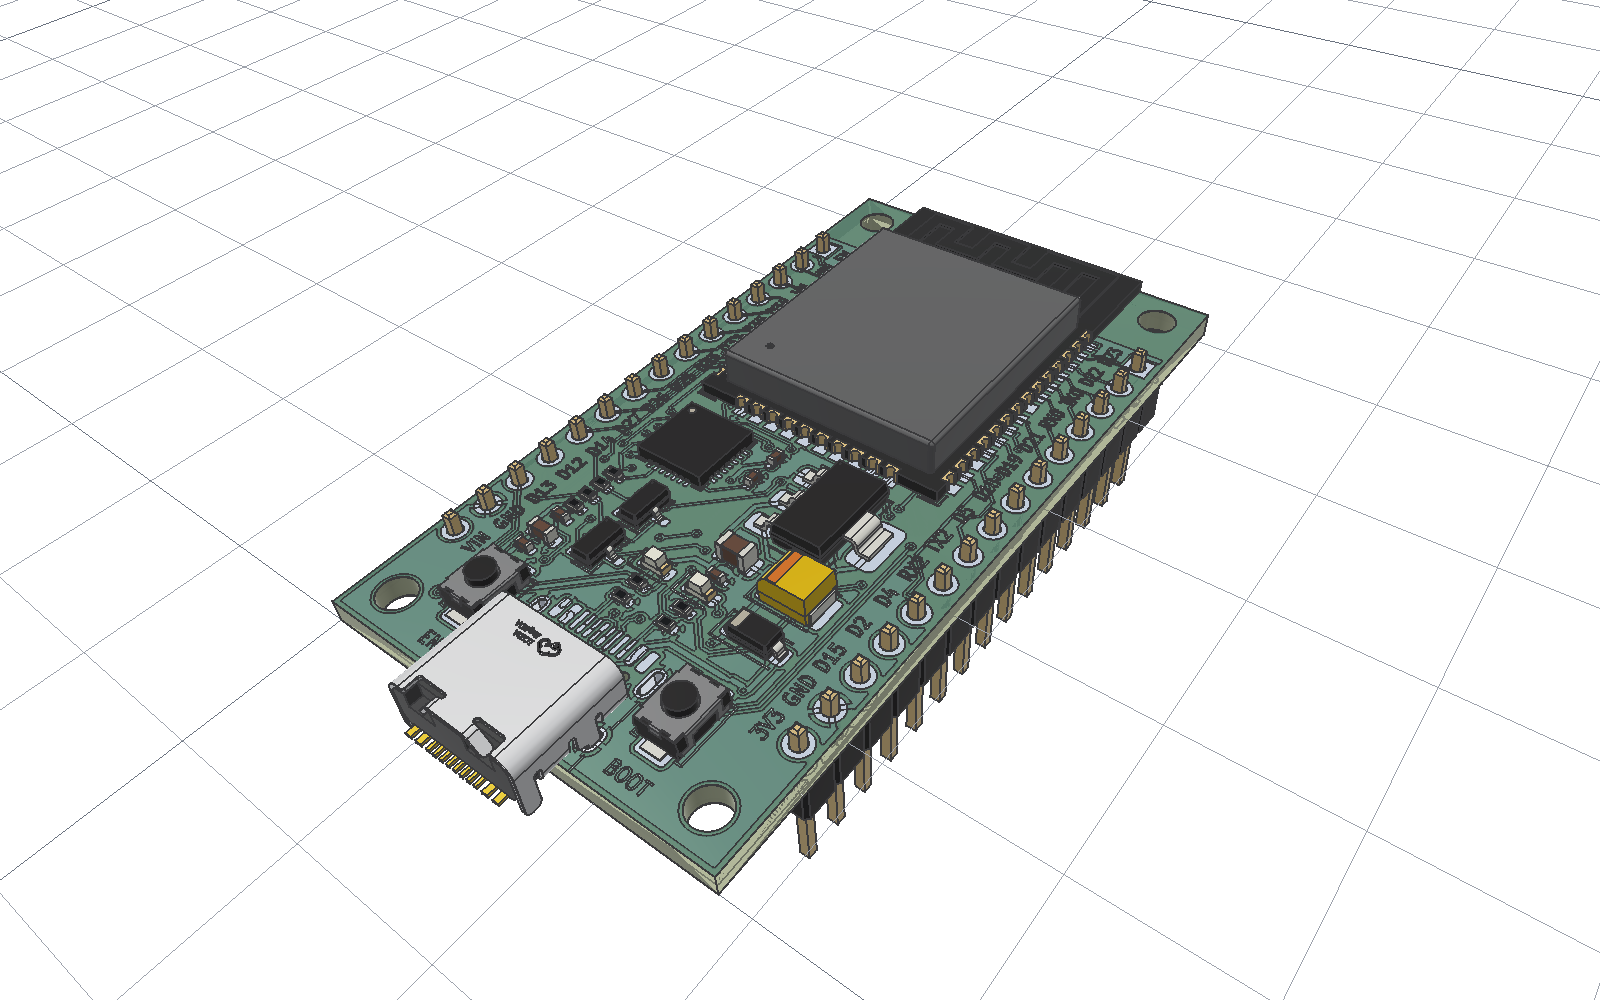
\includegraphics[width=0.60\linewidth]{fig/ecd05_board_3d.png}\hfill
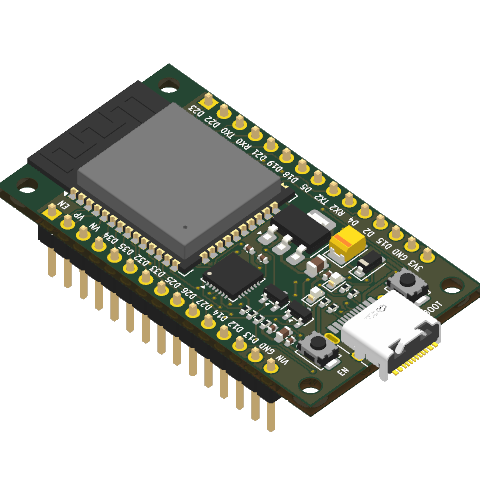
\includegraphics[width=0.37\linewidth]{fig/ecd05_thumbnail.png}\\[4pt]
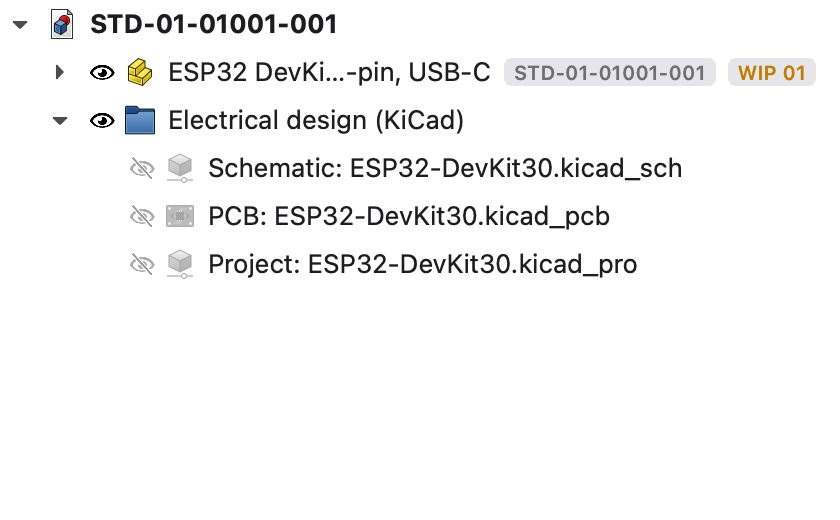
\includegraphics[width=0.55\linewidth]{fig/ecd05_tree.png}
\caption{A copy of the ESP32 DevKit (30-pin, USB-C) imported into a scratch Standard Libraries vault as
\code{STD-01-01001-001}. Top left: Open from Vault in Keystone (off-screen render of the real document, 37 bodies,
7.9\,g, FR-4, copper, epoxy, ceramic, PBT). Top right: KiCad's iso render, made at check-in and stored in the item as
its thumbnail. Bottom: the 3D model's Browser tree; the entries under \emph{Electrical design (KiCad)} open the
schematic, the PCB or the project in KiCad.}
\label{fig:ecd05-built}
\end{figure}

\paragraph{How a KiCad part lives in the vault.} A KiCad project is a folder, so each version is the folder packed into
one object, \file{<P/N>.kicad.zip}, and the work copy is the folder itself:
\begin{center}
\small
\begin{tabularx}{\linewidth}{@{}lX@{}}
\toprule
Where & What\\
\midrule
\file{objects/<ab>/<sha256>.zip} & one version: the project, deflated, entries sorted, fixed dates\\
\file{work/<you>/<P/N>/} & the work copy: \file{.kicad\_pro}, \file{.kicad\_sch}, \file{.kicad\_pcb}, project models
  and libraries, fab outputs, scripts\\
\file{\ \ keystone-part.json} & the part's description, manufacturer, MPN and value (travels with the version)\\
\file{\ \ thumbnails/Thumbnail.png} & KiCad's iso render; the Data panel reads it from the object as it does from an
  \file{.FCStd}\\
\file{\ \ .keystone/<P/N>.FCStd} & the board in 3D, made by Keystone, never checked in\\
\bottomrule
\end{tabularx}
\end{center}
Check-out, check-in (comment required), Undo Check-Out, Get Latest and Get Revision work on the folder: the files are
writable only while it is checked out to you, so KiCad opens a project that is not checked out read-only. The status
compares a \emph{tree digest}, $d = \mathrm{SHA256}\big(\sum_i \text{path}_i \,\|\, \mathrm{SHA256}(\text{file}_i)\big)$
over the sorted files, with the digest recorded when the version was put there, so the zip's bytes never matter and
what KiCad writes on its own (\file{*-backups/}, \file{fp-info-cache}, \file{*.lck}, \file{.history},
\file{\_autosave-*}, the local view settings \file{*.kicad\_prl}) never makes the part look modified. Check-in
renders the thumbnail again only when the board's content changed (cached by its hash, like the STEP export).

\paragraph{How you open it.}
\begin{itemize}[nosep]
  \item \textbf{3D in Keystone}: switch the Data panel to Standard Libraries and double-click the part (Open from
        Vault). The first open exports the board (about 20\,s for the ESP32 board); later opens take 2\,s. The model
        is made again when the board, the revision, the state or the part's values change. It carries the P/N,
        revision, description, type \code{cots}, manufacturer, MPN, value, materials and mass.
  \item \textbf{Electrical in KiCad}: right-click the part $\rightarrow$ \emph{Open in KiCad} (Data panel, or the
        Browser on a vault item), or double-click \emph{Schematic}, \emph{PCB} or \emph{Project} under
        \emph{Electrical design (KiCad)} in the 3D model. A WIP part nobody holds asks first: \emph{Check Out and
        Open} or \emph{Open Read-Only}. After editing in KiCad, \emph{Check In\ldots} as for any vault file.
  \item \textbf{In an assembly}: Insert Board on the part's \file{.kicad\_pcb} in the vault; the inserted board takes
        the part's P/N, revision and description, so the assembly BOM lists the library part on one line.
  \item \textbf{Import}: BruceWorx menu $\rightarrow$ \emph{Import KiCad Project as Standard Part\ldots} (pick the
        \file{.kicad\_pro}, fill in description, manufacturer, MPN, value, comment), or
        \code{bw-hooks vault kicad-import -{}-vault <Standard Libraries> -{}-from <project folder> -{}-comment "..."}
        (\code{-{}-dry-run} shows the P/N and the files first; \code{-{}-exclude build} leaves a folder out;
        \code{kicad-update} checks a newer copy in as the next version; \code{kicad-open} opens it in KiCad). The
        original folder is only read.
\end{itemize}

\paragraph{Decided while building} (the conservative choice each time; questions below).
\begin{itemize}[nosep]
  \item \textbf{No new item type.} The part is \code{cots}, the Standard Libraries' type; what makes it a KiCad part is
        its file (\file{.kicad.zip}). A new \code{pcb} type would make every older Keystone refuse the vault's
        journal. Consequence: a Keystone built before 30 Oct lists the part but cannot open it, so the real board goes
        in after Keystone is restaged.
  \item \textbf{The 3D model is derived, not versioned}, and sits inside the part's folder, not as \file{<P/N>.FCStd}
        beside the other work files: Keystone would otherwise treat it as the vault file (check-out offers, a lock
        on its tab). Assemblies take the board through Insert Board (a copy of the geometry with the part's P/N), not
        a link.
  \item \textbf{Manufacturer, MPN and value} are kept in the part (\file{keystone-part.json}) and shown as
        properties of its 3D part; the built-in part-property schema is unchanged.
  \item \textbf{Everything in the project folder goes in} (fab outputs, scripts, PDFs) except KiCad's own noise and
        caches; \code{-{}-exclude} leaves more out.
  \item \textbf{Import target}: the Standard Libraries vault beside the open vault (\code{Vault/Standard Libraries}),
        or the open vault when that is Standard Libraries; numbered like a part, \code{STD-01-\ldots}.
\end{itemize}

\paragraph{Tests.} Headless (\file{addons/BruceWorx/tests/test\_ecad\_vault.py}, 19 tests, 0.5\,s, KiCad's
Arduino~Mega template for the real-render case): project files and exclusions, deterministic packing, unpacking that
keeps KiCad's lock files and refuses unsafe names, import (number, type, comment, properties, missing models, the
thumbnail in the object, nothing left in staging, the source untouched, a second import of the same board refused),
check-out/edit/check-in, an unchanged check-in releasing the lock, KiCad's files not counting as edits, undo,
Newer and Get Latest, Get Revision, state across sessions, \code{kicad-update}, the three CLI actions with
\code{-{}-dry-run} and \code{-{}-exclude}, and the launch commands (nothing started). The pdm workspace, folder, CLI,
links, move, setup, dashboard, contract and project suites pass unchanged. FreeCAD
(\file{TestBruceWorxBoard.TestVaultItem}, headless and GUI): the item's 3D model with its values, read-only on disk,
the Electrical design entries resolving into the work folder, the freshness stamp, Insert Board taking the P/N; in
the GUI, Open from Vault opening the model (and not remaking it), Open in KiCad on the schematic with the check-out
offer, the vault menu's \emph{Open in KiCad}, the import form wanting a comment and \code{run\_import}. The
vault client's 30 GUI tests pass. Real check: a copy of the ESP32 project imported by the CLI into a scratch Standard
Libraries vault (18 files then, render included, 0.5\,s) and opened in Keystone (figure~\ref{fig:ecd05-built}); a
dry run against your real Standard Libraries vault (read only) names \code{STD-01-01002-001} and 51 files (37 without
\file{build/}).

\paragraph{Not done.} Update Board and the newer-version badge on a board in an assembly (the rest of ECD-05); a
KiCad mark on the part's row in the Data panel; a part whose work folder iCloud has evicted (your vault is on the
external disk); several KiCad projects in one folder (the import picks one by name).

\paragraph{Open questions for you.}
\begin{center}
\small
\begin{tabularx}{\linewidth}{@{}lXX@{}}
\toprule
\# & Question & Built for now (recommendation)\\
\midrule
1 & A KiCad part's item type: \code{cots} (as built) or a new \code{pcb}/\code{pcba} type? & \code{cots}: older Keystones
  keep reading the vault. Revisit when every Keystone is new.\\
2 & In assemblies: Insert Board (geometry copied, P/N carried) or a link to the part's 3D model, which would then have
  to be checked in with each version? & Insert Board; a link once Update Board (ECD-05) exists.\\
3 & Manufacturer, MPN and value: add them to the company part properties (every part gets them) or keep them on KiCad
  parts only? & KiCad parts only.\\
4 & Fab outputs (gerbers, STEP, BOM/CPL for JLCPCB) in the part, or left out by default? & In the part: the
  released revision then carries what was ordered.\\
\bottomrule
\end{tabularx}
\end{center}
